\documentclass[11pt]{article}
% Shared preamble for the notes in this repository. pdfLaTeX, TeX Live 2024 or later.
\usepackage[a4paper,margin=2.6cm]{geometry}
\usepackage[T1]{fontenc}
\usepackage{lmodern}
\usepackage{microtype}
\usepackage{amsmath,amssymb,amsthm}
\usepackage{graphicx}
\usepackage{booktabs}
\usepackage{enumitem}
\usepackage[dvipsnames]{xcolor}
\usepackage[hidelinks]{hyperref}
\hypersetup{colorlinks=true,linkcolor=MidnightBlue,citecolor=MidnightBlue,urlcolor=MidnightBlue}
\graphicspath{{../../figures/}}
\setlist{itemsep=2pt,topsep=4pt}

\newtheorem{theorem}{Theorem}
\newtheorem{proposition}[theorem]{Proposition}
\newtheorem{corollary}[theorem]{Corollary}
\newtheorem{conjecture}[theorem]{Conjecture}
\theoremstyle{definition}
\newtheorem{definition}[theorem]{Definition}
% Reusable derivations, numbered note.k; each note sets \notenumber. Indexed in DERIVATIONS.md.
\newcommand{\notenumber}{0}
\newtheorem{derivation}{Derivation}
\renewcommand{\thederivation}{\notenumber.\arabic{derivation}}
\newtheorem{question}{Question}
\theoremstyle{remark}
\newtheorem{remark}[theorem]{Remark}

\newcommand{\Z}{\mathbb{Z}}
\newcommand{\Q}{\mathbb{Q}}
\newcommand{\R}{\mathbb{R}}
\newcommand{\C}{\mathbb{C}}
\newcommand{\HH}{\mathbb{H}}
\newcommand{\SL}{\mathrm{SL}}
\newcommand{\Gal}{\mathrm{Gal}}
\newcommand{\Hom}{\mathrm{Hom}}
\newcommand{\repo}{\href{https://github.com/rmorleysmith/l-functions-and-physics}{\texttt{l-functions-and-physics}}}
\newcommand{\formal}{\href{https://github.com/rmorleysmith/morley-smith-formal}{\texttt{morley-smith-formal}}}
\newcommand{\script}[1]{\href{https://github.com/rmorleysmith/l-functions-and-physics/blob/main/scripts/#1}{\texttt{scripts/#1}}}
% A path inside the Lean repository; it may break after a slash.
\newcommand{\leanpath}[1]{\nolinkurl{#1}}

% Grades used in every status table.
\newcommand{\gradeLean}{\textsc{lean}}      % proved in Lean 4 with Mathlib
\newcommand{\gradeClassical}{\textsc{classical}}  % a published theorem, cited
\newcommand{\gradeComputed}{\textsc{computed}}    % checked numerically by a script in this repository
\newcommand{\gradeConvention}{\textsc{convention}}  % a choice of units or names
\newcommand{\gradeOpen}{\textsc{open}}      % a question, conjecture or working hypothesis
% The legend printed under every status table.
\newcommand{\gradelegend}{\par\nopagebreak\smallskip\noindent\begin{minipage}{\textwidth}\small
\gradeLean: proved in Lean 4 with Mathlib.
\gradeClassical: a published theorem.
\gradeComputed: checked numerically by a script in the repository \repo.
\gradeConvention: a choice of units or names.
\gradeOpen: a question, conjecture or working hypothesis.
\end{minipage}\par\medskip}
% A plain-language physical reading, placed after each derivation.
\newcommand{\physical}{\paragraph{In physical terms.}}


\title{How many colours in the rainbow?}
\author{Richard Morley-Smith}
\date{Note 03 \quad November 2026}

\begin{document}
\maketitle

\begin{abstract}
\noindent
Seven, by convention: Newton chose seven colours by analogy with the seven notes of the musical scale.
The visible spectrum is continuous, and colour vision is three-dimensional.
The visible band spans close to one octave of frequency: 1.97 with the common limits of 380--750\,nm, 2.31 with the colorimetric limits of 360--830\,nm.
The seven diatonic steps of that octave do not line up with the named colour bands.
Hydrogen, by contrast, has exact rational frequency ratios, because of the Rydberg formula.
Each series spans the ratio $(m+1)^2/(2m+1)$ from its first line to its limit: $4/3$ for Lyman and $9/5$ for Balmer.
We separate the exact statements from the labels.
\end{abstract}

\section{Seven by convention}

Newton divided the spectrum of white light into seven colours in the \emph{Opticks} (1704).
He compared their extents with the intervals of the musical scale.
Earlier divisions had used five colours, and Newton added orange and indigo \cite{Whipple}.
The physics gives no such division.
The spectrum is a continuum of wavelengths, and the eye samples it with three types of cone.
So perceived colour is a point in a three-dimensional space, not a position on a line.
The number of named colours varies between languages and conventions.

\section{The octave of light}

Frequency is inversely proportional to wavelength, so a band from $\lambda_1$ to $\lambda_2$ spans the frequency ratio $\lambda_2/\lambda_1$.
For 380--750\,nm this is $1.974$, just under an octave.
The CIE colour-matching tables run from 360 to 830\,nm, a ratio of $2.31$, just over one.
``The visible spectrum is an octave'' is therefore true only roughly, and depends on where the threshold is put.

Figure~\ref{fig:spectrum} sets three divisions of the octave side by side.
\begin{itemize}
\item The six conventional colour bands have widths 70, 45, 75, 20, 30 and 130\,nm.
\item The seven diatonic steps of the octave 750$\to$375\,nm have widths 82, 73, 33, 61, 55, 49 and 22\,nm.
\item The visible Balmer lines of hydrogen sit at 656.5, 486.3, 434.2 and 410.3\,nm (vacuum wavelengths).
\end{itemize}
The first two divisions do not correspond.

\begin{figure}[ht]
  \centering
  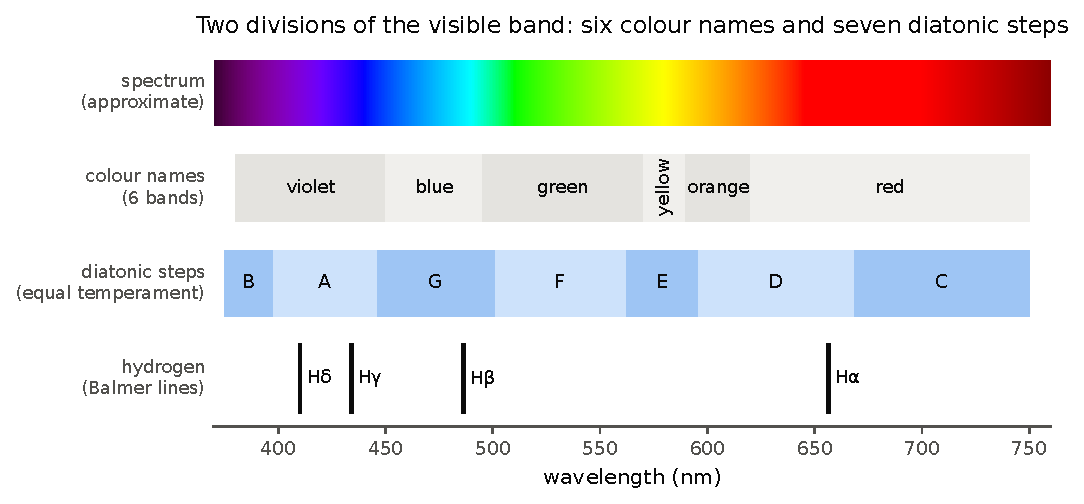
\includegraphics[width=0.95\textwidth]{light-spectrum}
  \caption{The visible spectrum (approximate sRGB rendering), the conventional colour names, the diatonic steps of the octave 750$\to$375\,nm, and the Balmer lines. Script: \script{light.py}.}
  \label{fig:spectrum}
\end{figure}

\section{Hydrogen: exact ratios}

The Rydberg formula $1/\lambda = R_H(1/m^2-1/n^2)$ makes every frequency ratio in the hydrogen spectrum rational.
In the Balmer series ($m=2$), consecutive visible lines have ratios
\[
  \tfrac{27}{20},\quad \tfrac{28}{25},\quad \tfrac{200}{189},\quad \tfrac{405}{392}.
\]
These are near musical intervals but not equal to them.
$\tfrac{27}{20}$ is 21.5 cents above the fourth $\tfrac43$, and $\tfrac{28}{25}$ is 7.7 cents below the tone $\tfrac98$.
The span of a whole series, from its first line $n=m+1$ to its limit $n\to\infty$, is exact:
\[
  \frac{1/m^2}{1/m^2 - 1/(m+1)^2} = \frac{(m+1)^2}{2m+1} = \tfrac43,\ \tfrac95,\ \tfrac{16}7,\ \tfrac{25}9\quad(m = 1,2,3,4).
\]
So the Lyman series spans exactly a perfect fourth, and the Balmer series exactly a just minor seventh.
These ratios are exact consequences of the Rydberg formula.
Calling them intervals is a choice of name, not a physical mechanism.

\section*{Status of the statements}

\begin{center}
\small
\begin{tabular}{@{}p{0.62\textwidth}l@{}}
\toprule
Statement & Grade\\
\midrule
Seven colours & \gradeConvention{} (Newton)\\
The visible band spans about an octave (1.97 or 2.31, by convention) & \gradeComputed\\
Diatonic steps do not match the colour bands & \gradeComputed\\
Balmer ratios; series spans $(m+1)^2/(2m+1)$ & \gradeClassical{} (Rydberg), \gradeComputed\\
\bottomrule
\end{tabular}
\end{center}

\begin{thebibliography}{9}
\bibitem{Whipple} Whipple Library, University of Cambridge, \emph{Isaac Newton (1642--1727)}, \url{https://www.whipplelib.hps.cam.ac.uk/node/216}.
\end{thebibliography}

\end{document}
